\section{First model}

The Jupyter notebook for this chapter can be viewed at \url{https://aka.klawr.de/srp\#5}.

\subsection{Project structure}

The project structure is an important part to test models efficiently and evaluate them against other models to determine the most powerful model.
\name{deepmech} is built using a modified version of the Cookiecutter Data Science \cite{drivendata2019} structure. It can be viewed at \url{klawr.github.io/deepmech}.

% % root
The root folder contains files such as the license for the entire project.
The project is licensed under the MIT license, which allows anyone to modify, distribute or use it for private and commercial use, but with no liability or warranty on my part.
In the root folder there is another file requirements.txt, which is part of the installation process and allows to replicate all the code handled in this project.

% % data
The "Cookiecutter Data Science" structure allows a clear division of the data into raw data (which must never be touched), intermediate data (which are the raw data, but which are modified, supplemented or altered in some way) and processed data (which are to be fed into the model via a training algorithm).

% % logs
Logs are created during training with \name{TensorBoard}\footnote{TensorBoard is the visualization toolkit of \name{TensorFlow}. The visualizations created with \name{TensorBoard} are shown later.} The logs are distinguished by a timestamp of the respective training run.

% % TODO models folder...

% % reports
A folder with all reports used in the project is located in the respective directory, including this article.
The notebook folder in reports for this project (abbreviated as \name{srp}) contains the code used to determine the best model.
Models are trained with \name{Jupyter-Notebooks}. \cite{Jupyter2019}. 
Jupyter Notebooks is an interactive Python code development editor that provides an easy way to efficiently write and test code.
All notebooks with corresponding code are located in the \name{notebooks} directory in the root directory of this project\footnote{\url{https://aka.klawr.de/srp\#6}}.

% % src
\name{src} contains all the code (except for the demos used in the reports) that was used in the development and training of the models. They range from scripts that create appropriate environments for training the models to data generation and augmentation.

\subsection{Loading data}

Before the training of the model can begin, the data must be loaded.
As mentioned, the data in this project is stored in the \name{raw} directory of the \name{data} directory.
It is good practice to never work directly with the raw data, so the beginning of each training session includes a preparation phase in which the raw data is copied to the \name{processed} data directory (with possible extensions or changes in intermediate steps).

Accordingly, the training of a model in this project always starts with the following code

\begin{lstlisting}
from os.path import join

raw = join('data', 'raw')
interim = join('data', 'interim')
processed = join('data', 'processed')
    
from src.training_env import reset_and_populate
    
reset_and_populate(raw, processed, [400, 0, 100])
\end{lstlisting}

For the first model, the raw data itself is sufficient; therefore, it is simply copied from \code{training\_env.py} to the directory of the processed data using a predefined function.
The third parameter of \code{reset\_and\_populate} is an array of three numbers describing the distribution of training, validation, and test data.
In this example, the validation data is omitted because no adjustments are made to the hyperparameters.

\begin{lstlisting}
from tensorflow.keras.preprocessing.image import ImageDataGenerator

def create_generator(data_dir, batch_size):
    datagen = ImageDataGenerator(rescale=1./255)
    full_path = join(processed, data_dir)
    return datagen.flow_from_directory(
        full_path,
        target_size=(32, 32),
        batch_size=batch_size,
        class_mode='binary')

train_generator = create_generator('train', 20)
test_generator = create_generator('test', 10)
\end{lstlisting}

After the corresponding directories are filled with data, the \code{ImageDataGenerator}\footnote{\url{https://keras.io/preprocessing/image}} is used to allow the model to load the data later during the training process.
The generators also define the size of the loaded image, which can be set to 32 pixels wide and 32 pixels high (as opposed to the original image size of 512x512) and a batch size\footnote{batch size is the number of images used between each backpropagation cycle.
If the batch size matches the record size, it is called batch gradient descent, if the batch size is one, it is called stochastic gradient descent.
Everything in between is called a mini-batch gradient descent.} of 20.
The \code{class\_mode} is set to \code{binary} because the input consists of 1D Numpy arrays.
These generators also recognize the structure of the raw data (distributed in respective directories using their label as directory name) and thus assign the appropriate labels to them.

\subsection{Creation of the model}

\begin{lstlisting}[label={lst:first_model}]
from tensorflow.keras import layers
from tensorflow.keras import models

model = models.Sequential()
model.add(layers.Flatten(input_shape=(32, 32, 3)))
model.add(layers.Dense(32,'relu'))
model.add(layers.Dense(32,'relu'))
model.add(layers.Dense(3, 'softmax'))

model.summary()
\end{lstlisting}

All models used in this project are sequential models.
Sequential models propagate the result of each layer in one direction to the next layer.

\name{Keras} requires that the first layer has a \code{input\_shape}.
The input shape of the first model must match the actual size of the input data.
All other layers are able to derive the shape of the previous layer, so no further definitions are required.

Layers can be added by using a provided \code{add} function which accepts layers as parameters which are subsequently added to the model.

Layers can be added using a provided \code{add} function that accepts layers as parameters, which are then added to the model.

Two layers are added, both of which are dense layers with 32 nodes each.
The dense layers are defined by connecting all nodes of the previous layer to the nodes of their own layer using weights and biases and behave like the "traditional" layers used in this project.
The two hidden layers are activated with the \name{ReLU} activation, as suggested in \cite[p.168]{Goodfellow2017}.

The last layer has three nodes in relation to three classes to which the data can be assigned.
The activation \name{softmax} is used, which adjusts the values of the layer so that they add up to the value one.
Therefore, the value of the node in the initial layer can be considered a measure of the confidence of the model's evaluation for a given input.
The node with the highest value is accordingly assumed to be the assumed correct result.

A summary of the model is given as:

\begin{lstlisting}
Model: "sequential"
_________________________________________________________________
Layer (type)                 Output Shape              Param #   
=================================================================
flatten (Flatten)            (None, 3072)              0         
_________________________________________________________________
dense (Dense)                (None, 32)                98336     
_________________________________________________________________
dense_1 (Dense)              (None, 32)                1056      
_________________________________________________________________
dense_2 (Dense)              (None, 3)                 99        
=================================================================
Total params: 99,491
Trainable params: 99,491
Non-trainable params: 0
_________________________________________________________________
\end{lstlisting}

Here we see that the model 99491 has parameters in $\theta$ that can be adjusted.
This number is the sum of the parameters given by the 3 layers of the model.
The first layer has the flattened 3072 ($32 \times 32 \times 3$) nodes.
The second layer multiplies this number (+1 for the bias) by $32$ and therefore has an additional 98336 nodes.
The third layer is the product of $32 + 1$ nodes in the second layer and $32$ nodes in the third layer, which gives us 1056 parameters to adjust.
The last layer again has $(32 + 1) \times 3$ nodes.

\subsection{Optimizer}

In order to train our model, an optimizer must be defined.
We will start with a \code{SGD} optimizer, which is the abbreviation for \name{Stochastic Gradient Descent}.
Stochastic gradient descent is already mentioned in chapter~\ref{ch:simple_linear_example}, where it was implemented very rudimentarily. In the actual training of the model, the Keras implementation is used.
The Keras implementation of SGD differs somewhat from the general definition, since it does not inherently assume a batch size of one, but rather the batch sizes defined in the respective generator, so that the user can decide whether to use full batch, mini batch, or stochastic gradient descent (which in this case is 20).

\begin{lstlisting}
    optimizer = SGD(lr=0.01, momentum=0.9, nesterov=True)
\end{lstlisting}

The function \code{SGD} requires three parameters: The learning rate \code{lr}, \code{momentum} and \code{nesterov}.
These values in turn are hyperparameters that must be determined before training.

\subsubsection{Learning rate}

The learning rate is one of the most influential hyperparameters and probably the most significant, since it is used in almost every optimizer.
It is a scalar value that determines the step size of the steps performed. The update function of the parameter $\theta$ is as already mentioned:

\begin{equation}
    \theta_{i+1} := \theta_i - \eta \varDelta \tag{\ref{eq:backprop_update} revisited}
\end{equation}.

Where $\eta$ is the value of the learning rate.

If the learning rate is set too low, the loss function needs many iterations to converge to a sufficiently low value.
On the other hand, a learning rate set to a high value cannot converge at all.

\begin{figure}
    \centering
    \begin{subfigure}[b]{0.3\textwidth}
        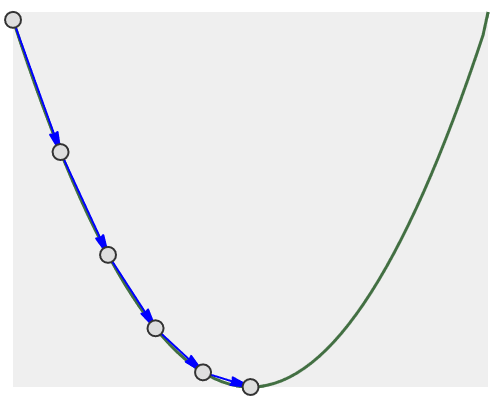
\includegraphics[width=\textwidth]{images/lr_ok.png}
        \caption{Learning rate just right}
        \label{fig:lr_ok}
    \end{subfigure}
    \begin{subfigure}[b]{0.3\textwidth}
        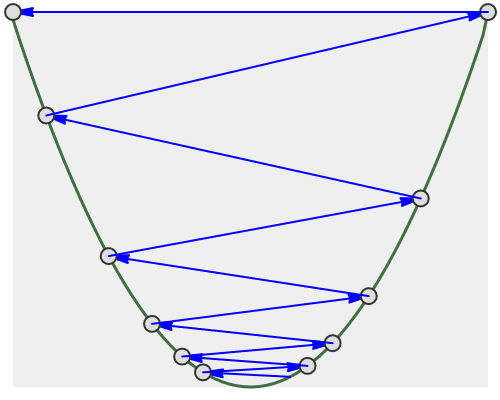
\includegraphics[width=\textwidth]{images/lr_too_high.png}
        \caption{Learning rate too high}
        \label{fig:lr_too_high}
    \end{subfigure}
    \begin{subfigure}[b]{0.3\textwidth}
        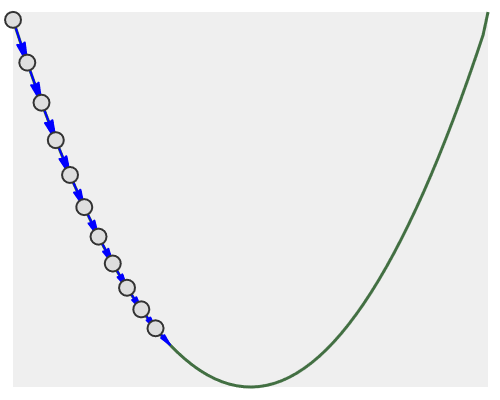
\includegraphics[width=\textwidth]{images/lr_too_low.png}
        \caption{Learning rate too small}
        \label{fig:lr_too-low}
    \end{subfigure}
    \caption{If the learning rate is just right, the value of the loss function approaches a local optimum in an acceptable number of steps.
    If it is too high, it diverges.
    If the learning rate is too low, the values converge, but too many steps are needed to achieve this.
    Please note that these pictures show the parameter space in a very simplified way, since the function shown is completely convex and only two-dimensional.}
    \label{fig:learning_rate}
\end{figure}

\subsubsection{Momentum}

Introduced in 1964 by Polyak \cite{Polyak1964}, momentum is used to keep the gradient constant over several steps.
Momentum takes its name as an analogy to the physical effect according to Newton's second law of motion.
The direction of correction by the gradient should be consistent over several steps, and it would be strange if the direction made sudden shifts during training.
This is useful if the data is "noisy" or some of the training examples are wrong.
Therefore another parameter $\nu$ is introduced into the equation~\eqref{eq:backprop_update}:

\begin{equation}
    \begin{split}
        \nu_{i} &:= \alpha \nu_{i-1} - \eta \varDelta \\
        \theta_{i+1} &:= \theta_i + \nu_i
    \end{split}
    \label{eq:momentum}
\end{equation}

In contrast, $\alpha$ is another parameter that can be set to regulate the influence of $\eta$ on the parameters of the next iteration.
Thus, if a training example would change the "direction" of the next step with a high deviation from the median of the last steps, the effect would be reduced and the convergence rate might be improved. 

In 2013 Sutskever, Martens, Dahl and Hinton \cite{Sutskever2013} introduced another variant of the momentum inspired by Nesterov's Accelerated Gradient \cite{Nesterov1983}.
This variant updates the previously discussed equation to change the parameter for calculating $\varDelta$ using $\nu$.
Please note that $\varDelta$ in equation~\eqref{eq:momentum} and ~\eqref{eq:backprop_update} is itself a function of the $\theta$ parameter (see equation~\eqref{eq:hidden_error}).

\begin{equation}
    \begin{split}
    \nu_i & := \alpha \nu_i - \eta \varDelta(\theta_i + \alpha \nu_i) \\
    \theta_{i+1} & := \theta_i + \nu_i
    \end{split}
    \label{eq:nesterov}
\end{equation}

The idea of momentum is that the direction vector points in the right direction, whereas the use of the Nesterov Accelerated Gradient is probably more accurate when one starts measuring the next error, which is slightly shifted in the respective direction \cite[p.353]{Geron2019} \cite[p.291]{Goodfellow2017}.

\subsubsection{Actual training}

After the optimizer is defined, the model is compiled by calling the model compile function.

\begin{lstlisting}
model.compile(
    loss='sparse_categorical_crossentropy', 
    optimizer=optimizer,
    metrics=['acc'])
\end{lstlisting}

\code{sparse\_categorical\_crossentropy} is used as a loss function, as recommended for multiclass categorization problems that are characterized by integers \cite[p.84]{Chollet2017}.
It measures the distance between two probability distributions given by the last layer of the model given by a \code{softmax} activation and the labelled data.
The SoftMax activation is used to normalize the output by dividing each value by the sum of all values in each layer.
This is useful because the labeled data assigns the value one to the correct node and zero to all others, making them numerically comparable and minimizing loss for a meaningful result.

The actual training then takes place using a \code{fit} function in the model.
The training data is provided by generators; the function in this case is \code{fit\_generator}.
Therefore, the training is performed by calling the following function:

% TODO python and remove generator
\begin{lstlisting}
history = model.fit_generator(
    train_generator,
    steps_per_epoch=20,
    epochs=20,
    callbacks=callbacks)
\end{lstlisting}

Here it is defined that 20 images are fed into the model as a batch at each iteration, which is repeated for 20 epochs.
Since an epoch is a run, the optimizer updates the parameters (the $\theta$ of the model) 20 times.

\subsubsection{Results}
\begin{figure}
    \centering
    \begin{subfigure}[b]{0.4\textwidth}
        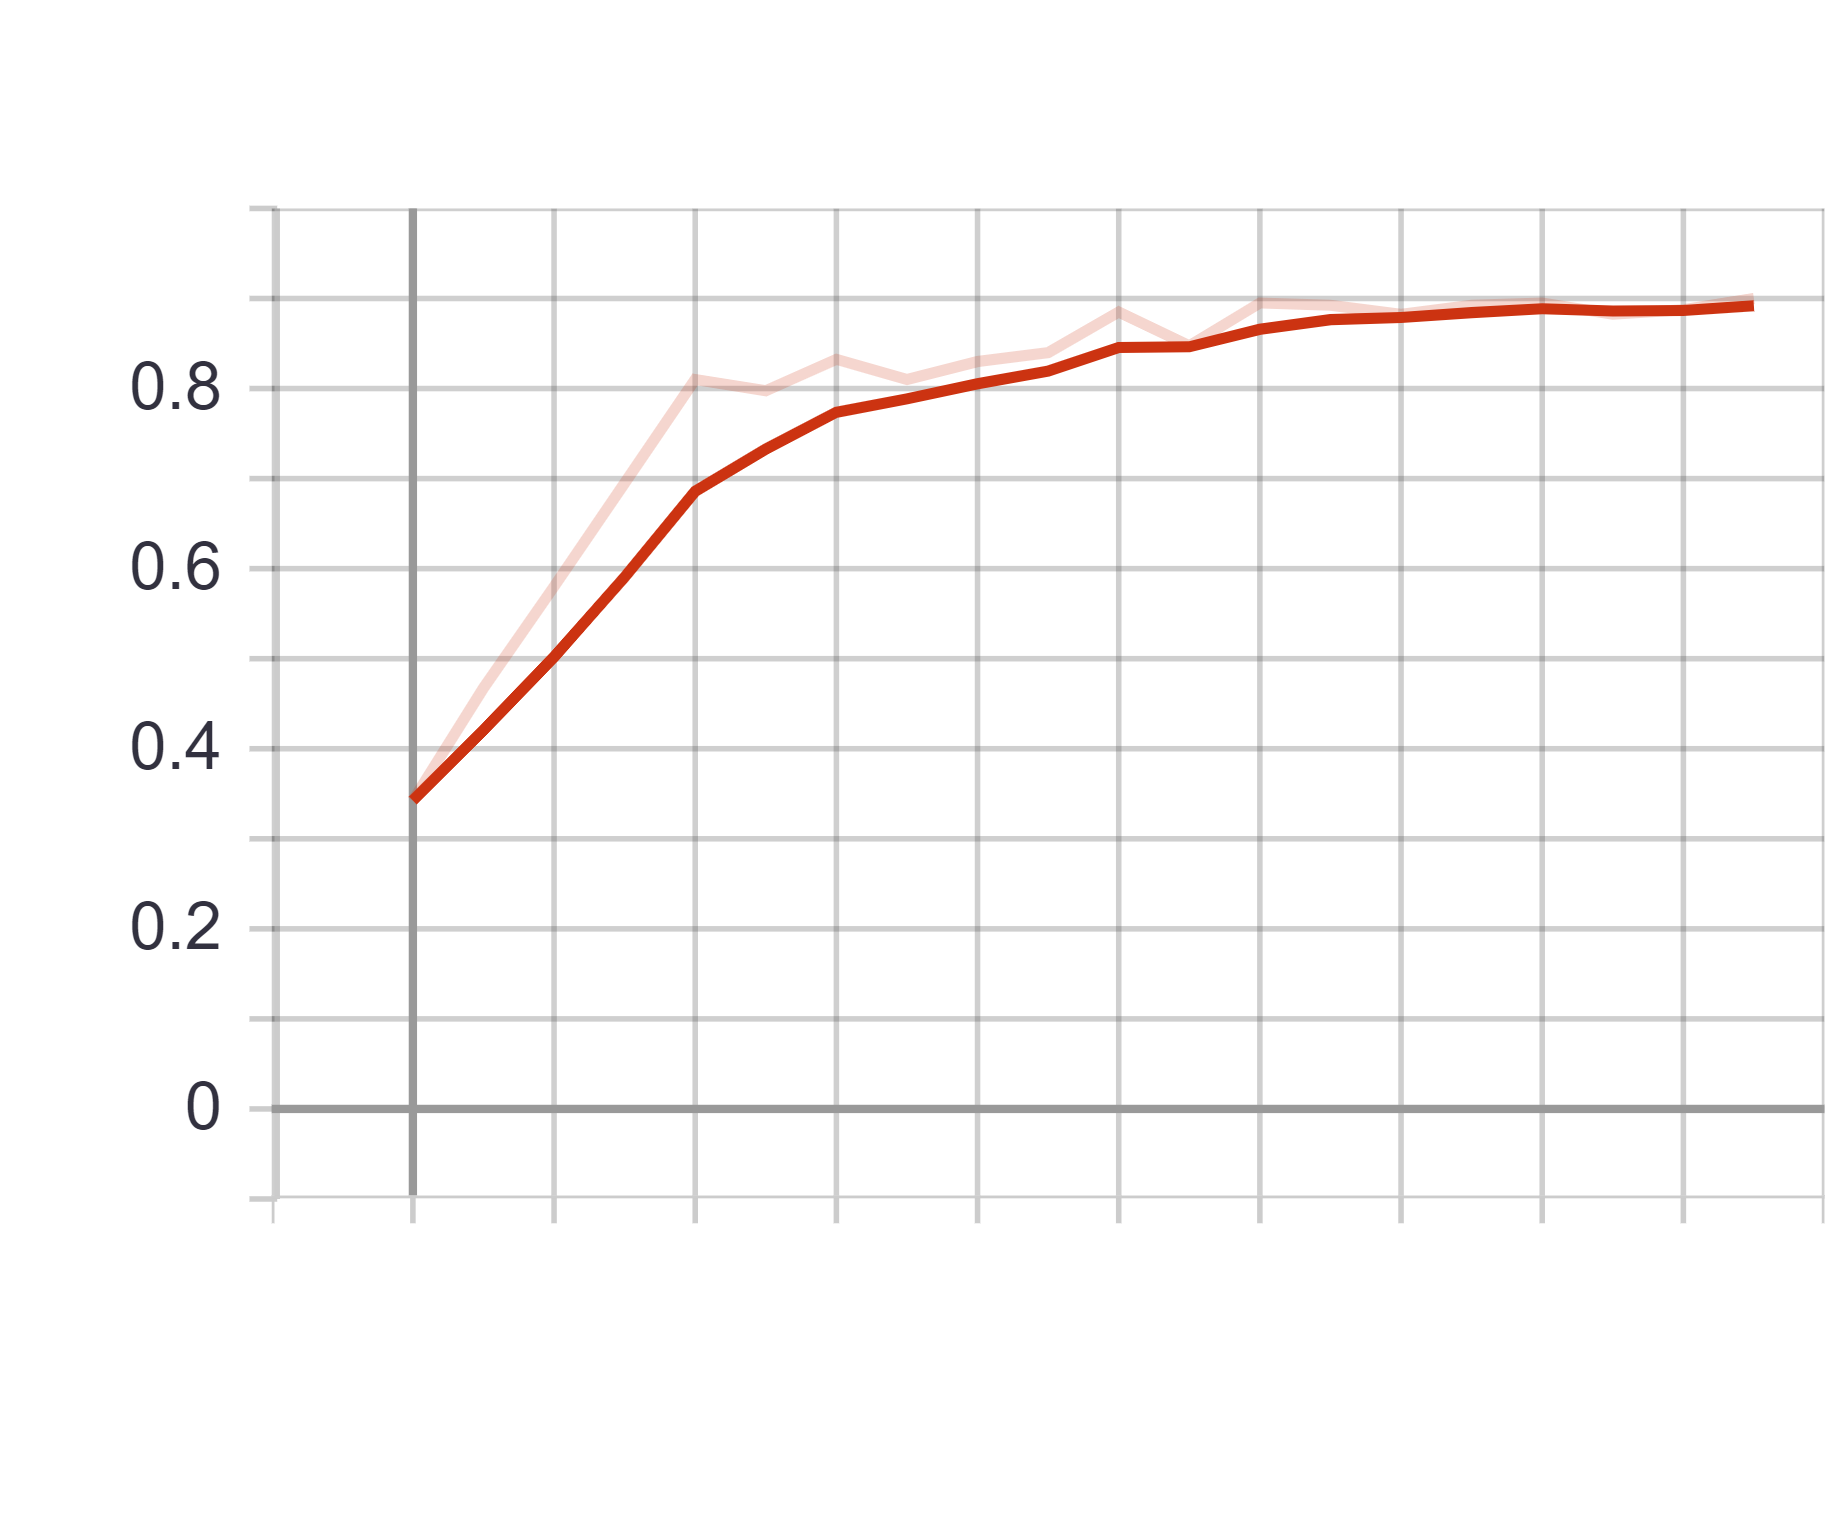
\includegraphics[width=\textwidth]{images/first_model_acc.png}
        \caption{Accuracy}
        \label{fig:first_model_acc}
    \end{subfigure}
    \begin{subfigure}[b]{0.4\textwidth}
        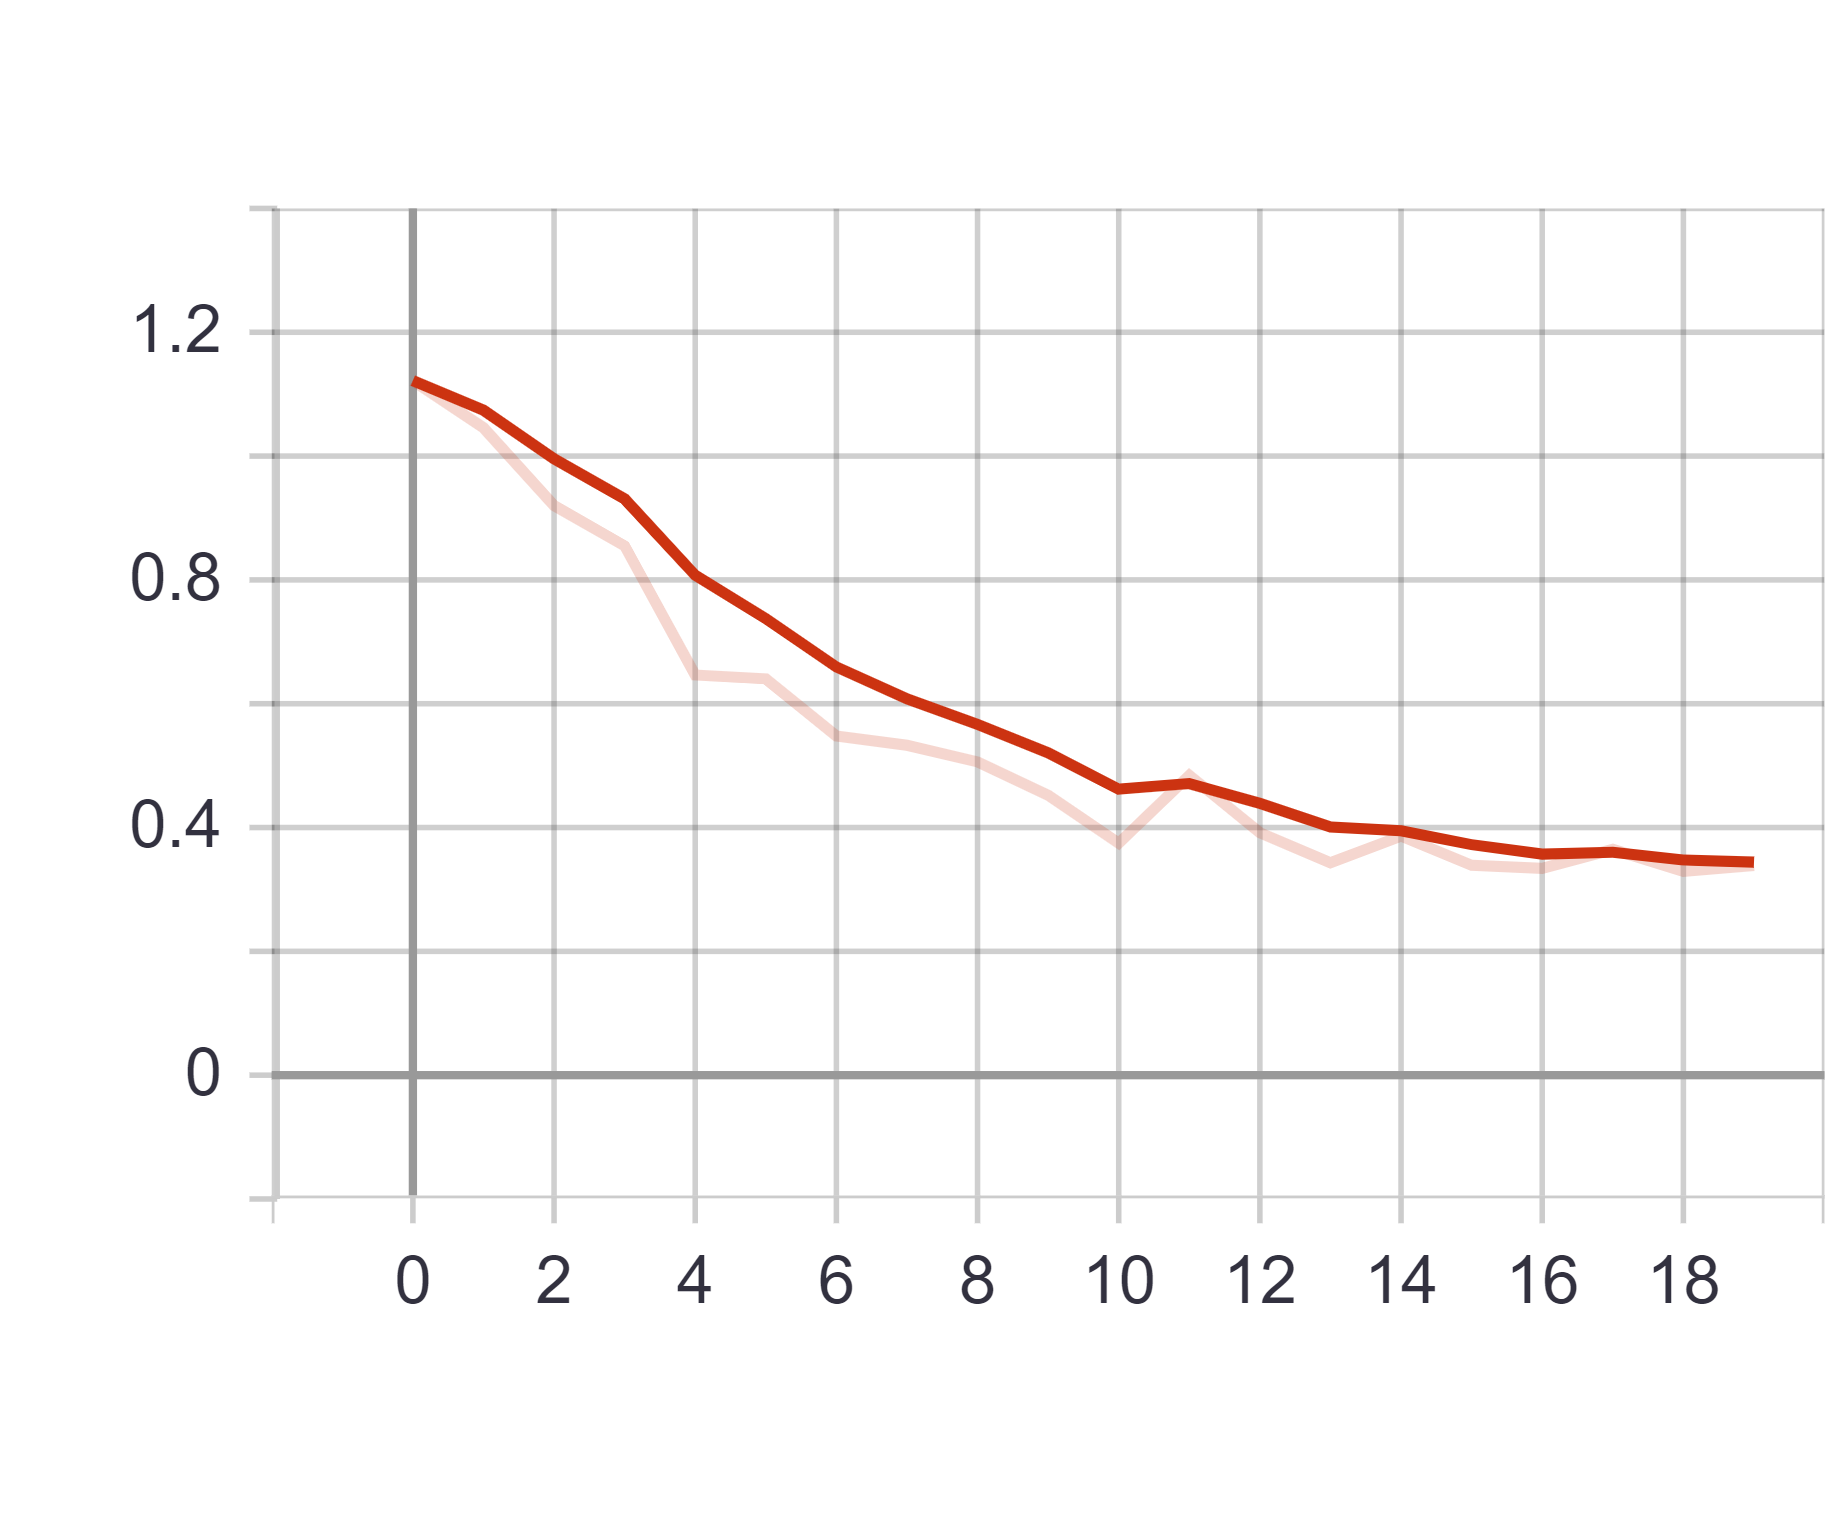
\includegraphics[width=\textwidth]{images/first_model_loss.png}
        \caption{Loss}
        \label{fig:first_model_loss}
    \end{subfigure}
    \caption{The callbacks of the training algorithm provide logs that can be used by TensorBoard to provide useful graphics for evaluating the model. The vertical axis represents the value of each epoch (shown on the horizontal axis).}
    \label{fig:first_model_graphs}
\end{figure}

As expected, the model starts with an accuracy of about 33\% by trying to classify the training data into three classes.
As the data suggests, the model quickly learns some relationships between the input data and the label, as it already has an accuracy of almost 70\% after only four epochs.

\begin{lstlisting}
Epoch 1/20
20/20 [=====...=====] - 2s 79ms/step - loss: 1.1220 - acc: 0.3425
Epoch 2/20
20/20 [=====...=====] - 1s 55ms/step - loss: 1.0457 - acc: 0.4675
Epoch 3/20
20/20 [=====...=====] - 1s 55ms/step - loss: 0.9199 - acc: 0.5800
Epoch 4/20
20/20 [=====...=====] - 1s 46ms/step - loss: 0.8548 - acc: 0.6950
...
Epoch 17/20
20/20 [=====...=====] - 1s 45ms/step - loss: 0.3340 - acc: 0.8950
Epoch 18/20
20/20 [=====...=====] - 1s 48ms/step - loss: 0.3648 - acc: 0.8825
Epoch 19/20
20/20 [=====...=====] - 1s 52ms/step - loss: 0.3291 - acc: 0.8875
Epoch 20/20
20/20 [=====...=====] - 1s 47ms/step - loss: 0.3388 - acc: 0.9000
\end{lstlisting}

After 20 epochs the model has an accuracy of about 90\%, which is already a very good start for a first model with non-optimized hyperparameters.
Important for a working model is how well the model classifies data it has never seen before.
To verify this, a second generator is created: the \code{test\_generator}, which is used to evaluate the model.
By outputting \code{model.evaluate\_generator(test\_generator)} we get \code{[0.6071663084129493, 0.7866667]}, which indicates that the loss is \code{0.60}, as opposed to \code{0.33} for the training data, and has an accuracy of 78\% on the data it has never seen before.

This result is quite remarkable, but obviously the model performs worse on new data, indicating that it overfitted on training data.
Regardless, the result shows that by adjusting the hyper parameters, the result should be able to be increased to a satisfactory level.

The model is then saved at \name{models/symbol\_classifier/first\_model.h5} and can be loaded into Keras for further review.